\chapter{Documento di design}
In questa sezione vengono illustrate le scelte architetturali e i design pattern adottati nel software.
Un design pattern è una soluzione generale e collaudata per risolvere problemi ricorrenti che si incontrano durante la progettazione di software.
Questi pattern possono migliorare la comprensione del codice, la manutenzione e la scalabilità di un'applicazione.

\bigskip\bigskip

\section{Architettura del Software}
L'architettura del software è suddivisa tra il client e il server, con il client sviluppato in Flutter e il server utilizzando AWS.

\subsection{Client}
L'applicazione client è sviluppata utilizzando Flutter, un framework open-source di Google per la creazione di applicazioni mobili nativamente compilate. Flutter consente di creare un'interfaccia utente ricca e reattiva, mantenendo un'alta performance sia su Android che iOS.\meskip
Il client sarà responsabile della visualizzazione dei dati e dell'interazione con l'utente.\\
La gestione dello stato sarà gestito tramite il pattern MVC (Model-View-Controller) integrato con i DAO (Data Access Object). 
Questo approccio separa la logica di business, la gestione dello stato e l'accesso ai dati, migliorando la manutenibilità e la testabilità del codice.

\subsection{Server}
Per la gestione del server, abbiamo scelto Amazon Web Services (AWS), una piattaforma cloud che offre un'ampia gamma di servizi, tra cui elaborazione, archiviazione, e database. 
Il server è stato implementato utilizzando un'istanza EC2, con un database gestito tramite RDS e la logica applicativa eseguita su un backend sviluppato in Express.


\subsection{Interazione tra Client e Server}
Il client invia richieste HTTP al backend seguento l'architettura REST. Il server riceve queste richieste, le elabora, e interagisce con il database per ottenere o aggiornare i dati.

Le risposte vengono restituite al client in formato JSON, garantendo così una facile integrazione e manipolazione dei dati all'interno dell'applicazione Flutter. 

La comunicazione tra client e server avviene attraverso richieste asincrone, che permettono al client di ottenere dati aggiornati in tempo reale senza interrompere l'esperienza dell'utente.

\section{Design pattern utilizzati}

\subsection{Model-View-Controller (MVC)}
Il pattern Model-View-Controller (MVC) è stato scelto per strutturare l'applicazione in modo da separare le responsabilità e facilitare la manutenzione del codice.

\begin{itemize}
	\item \textbf{Model}: Gestisce i dati dell'applicazione ed è responsabile della notifica alla View quando i dati cambiano. Questo permette alla View di aggiornarsi e riflettere le modifiche senza dover essere a conoscenza dei dettagli di come i dati sono gestiti.

	\item \textbf{View}: Si occupa della presentazione e dell'interfaccia utente. Mostra i dati agli utenti e aggiorna la visualizzazione in risposta alle modifiche del Model.

    \item \textbf{Controller}: Funziona da intermediario tra il Model e la View. Gestisce gli input degli utenti e aggiorna il Model e la View di conseguenza.
\end{itemize}

\subsection{Data Access Object (DAO)}
Il Data Access Object (DAO) è stato implementato per separare la logica di accesso ai dati dalla logica di business, semplificando la gestione e l'accesso ai dati.

\newpage

\section{Analisi delle scelte tecnologiche utilizzate}
\subsection{Client: Confronto con altre tecnologie}
La decisione di utilizzare flutter è stata presa dopo un'analisi delle opzioni disponibili, considerando vari fattori come la produttività, le prestazioni e la compatibilità.

\subsubsection{React Native}
\begin{itemize}
    \item \textbf{Prestazioni:} Flutter compila il codice direttamente in codice nativo, mentre React Native utilizza un ponte per comunicare tra JavaScript e codice nativo. Questo può portare a prestazioni superiori in Flutter.
    \item \textbf{Coerenza dell'UI:} Flutter utilizza un motore di rendering proprietario, che garantisce una coerenza visiva su tutte le piattaforme, mentre React Native si basa sui componenti nativi, il che può comportare variazioni tra iOS e Android.
\end{itemize}

\subsubsection{Sviluppo nativo (Java/Kotlin per Android, Swift per iOS)}
\begin{itemize}
    \item \textbf{Cross-Platform:} Flutter consente di scrivere un solo codice per entrambe le piattaforme, riducendo i tempi e i costi di sviluppo rispetto alla scrittura di codice separato.
    \item \textbf{Consistenza dell'Interfaccia:} Flutter offre un controllo totale sul rendering e sulla consistenza dell'interfaccia su entrambe le piattaforme.
    \item \textbf{Aggiornamenti e Manutenzione:} La manutenzione di una singola codebase è generalmente più semplice e meno costosa.
\end{itemize}

\subsection{Server}
\subsubsection{Amazon EC2}
\textit{Amazon Elastic Compute Cloud} (EC2) è il servizio di AWS che fornisce capacità di calcolo nel cloud. 
Tramite EC2, è possibile eseguire istanze di macchine virtuali configurabili in base alle esigenze del progetto, garantendo flessibilità e controllo totale sull'infrastruttura server.

Nel nostro caso, abbiamo implementato un server \textit{NodeJS} che esegue un backend \textit{express}.

\subsubsection{Amazon RDS}
\textit{Amazon Relational Database Service} (RDS) è il servizio gestito di AWS per database relazionali, che semplifica le attività di configurazione, gestione e scalabilità dei database. 

Nel nostro caso, abbiamo impiegato RDS con un database PostgreSQL.

\subsubsection{Express.js}
\textit{Express.js} è un framework per applicazioni web Node.js, utilizzato per sviluppare la logica applicativa del nostro backend. Ci ha permesso di implementare un'API RESTful in modo rapido ed efficiente, gestendo le richieste tra il client e il server e interfacciandosi con il database ospitato su RDS.

\section{Diagrammi di Sequenza di Design}
\subsection{Caso d'uso: Creazione Asta Silenziosa}
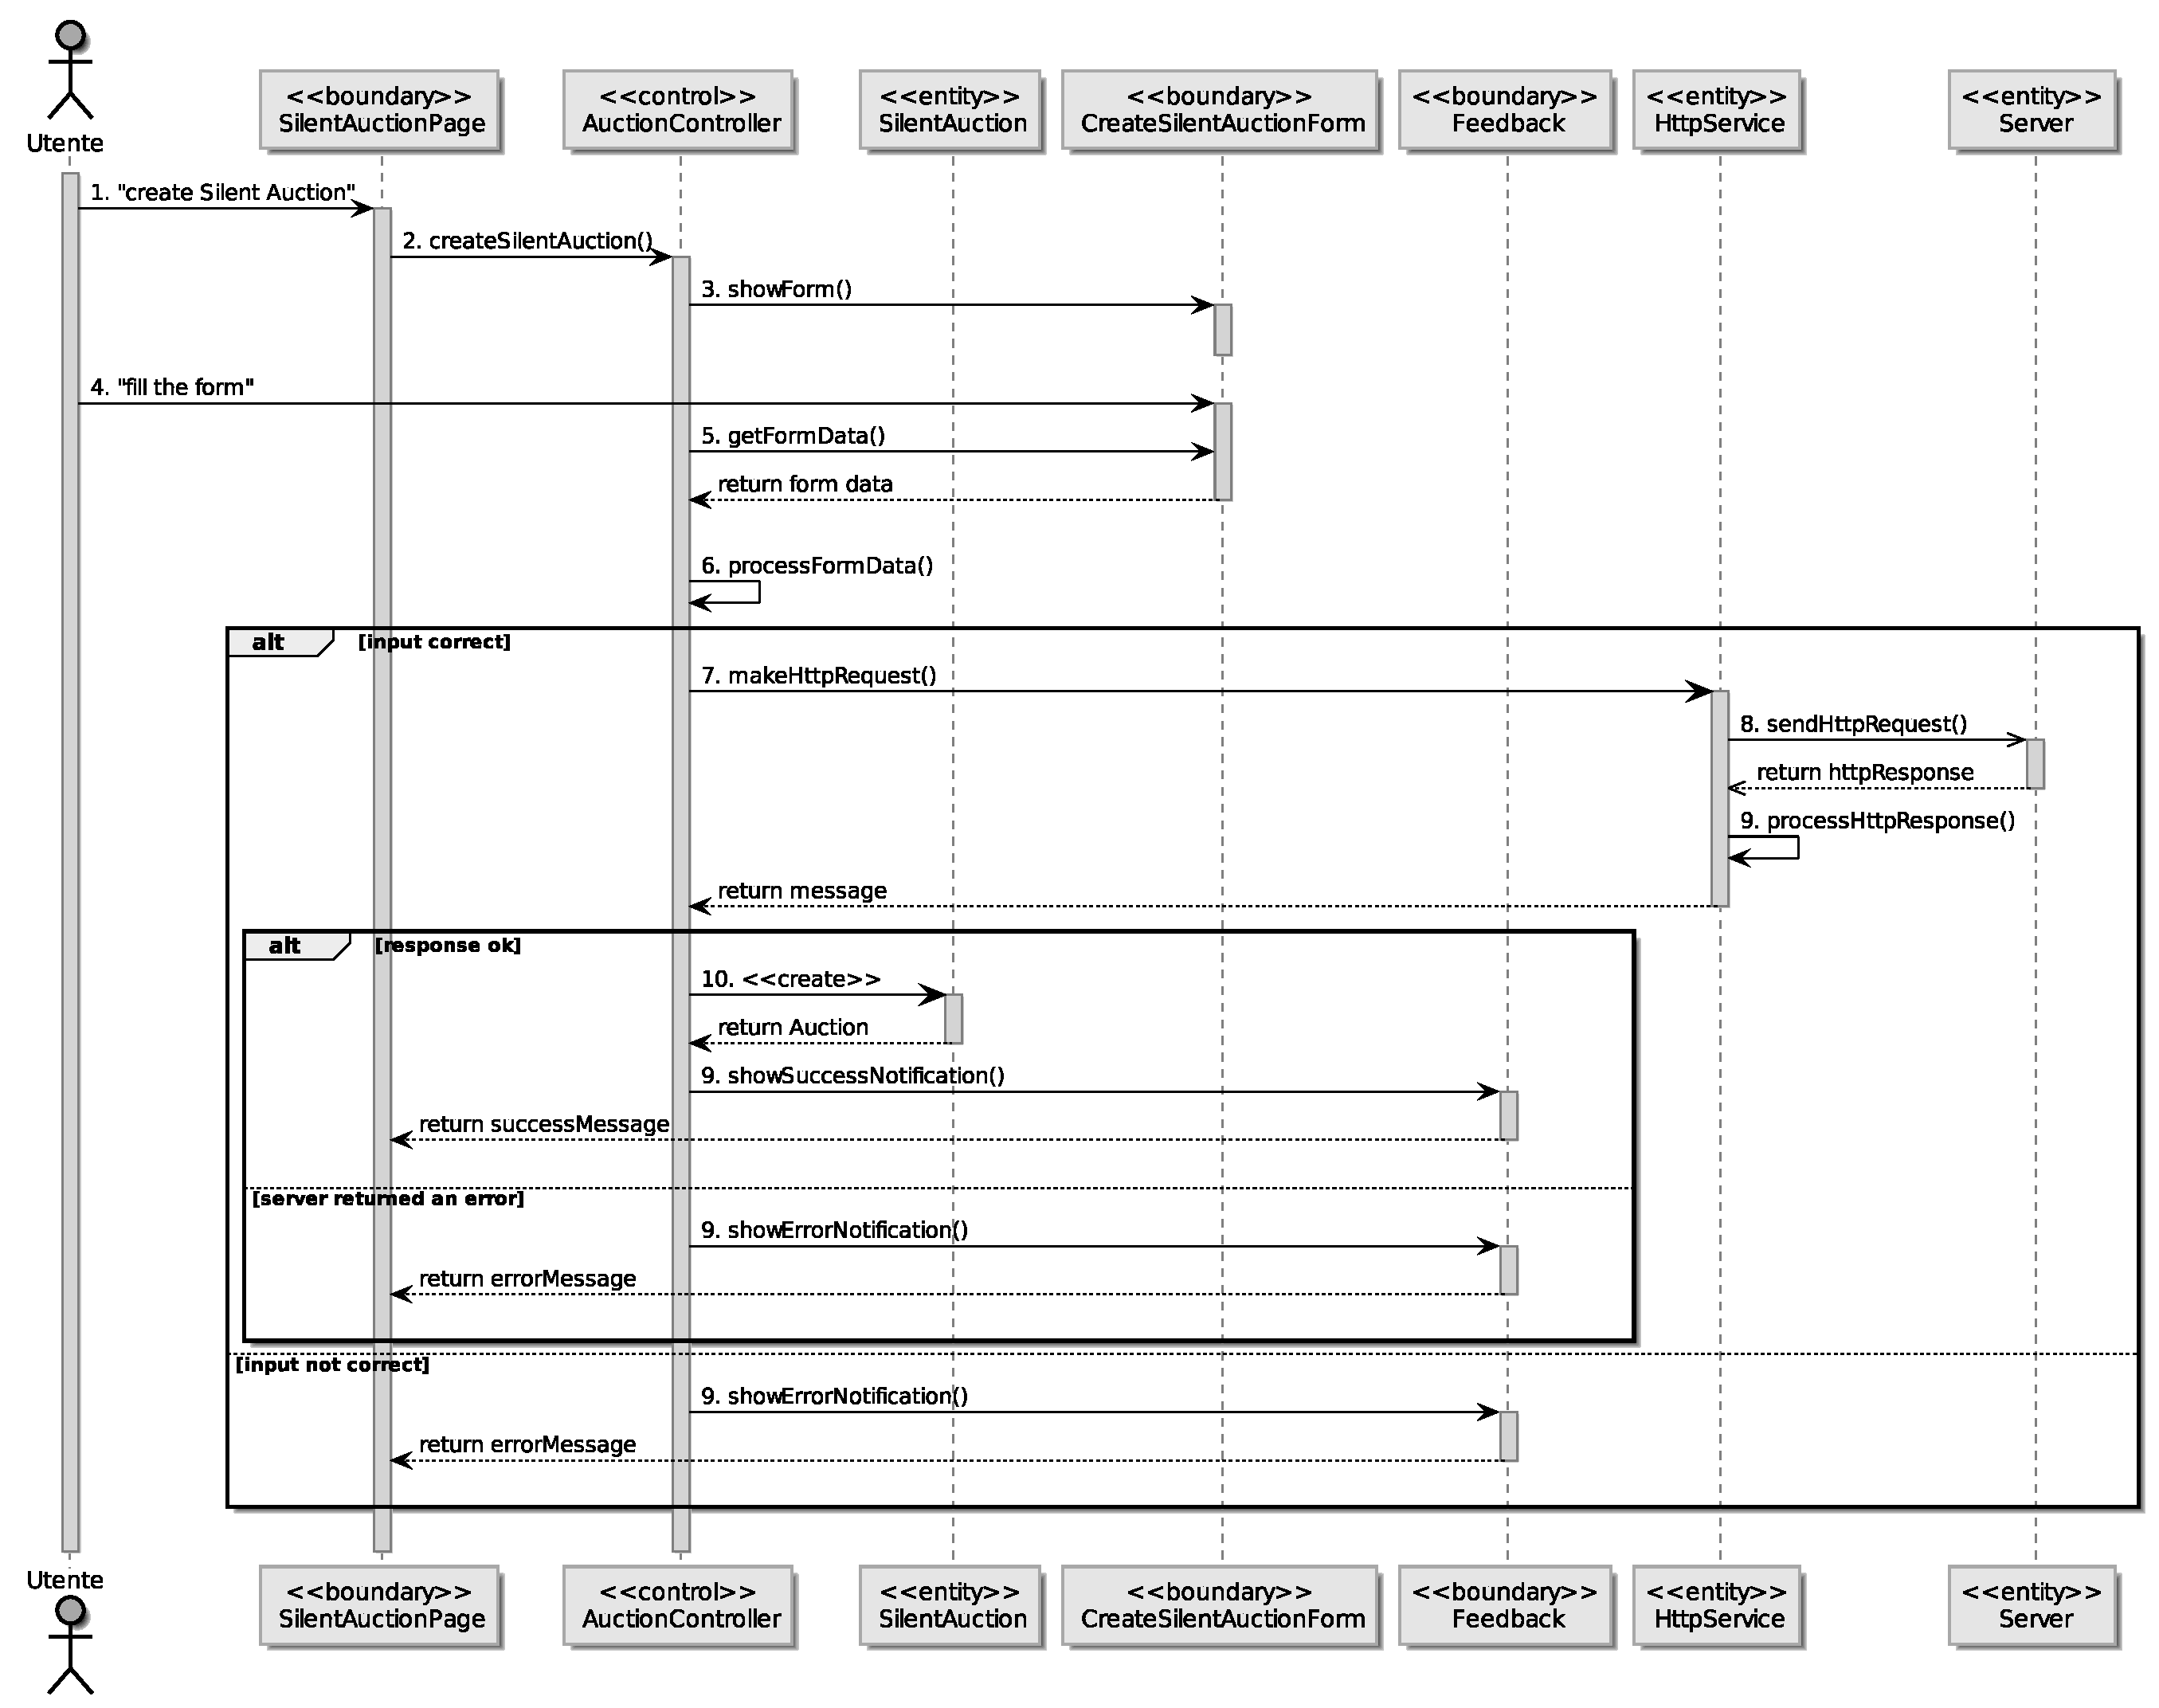
\includegraphics[width=\textwidth]{assets/sequence/creazione_asta_silenziosa.eps}

\subsection{Caso d'uso: Offerta Asta Silenziosa}
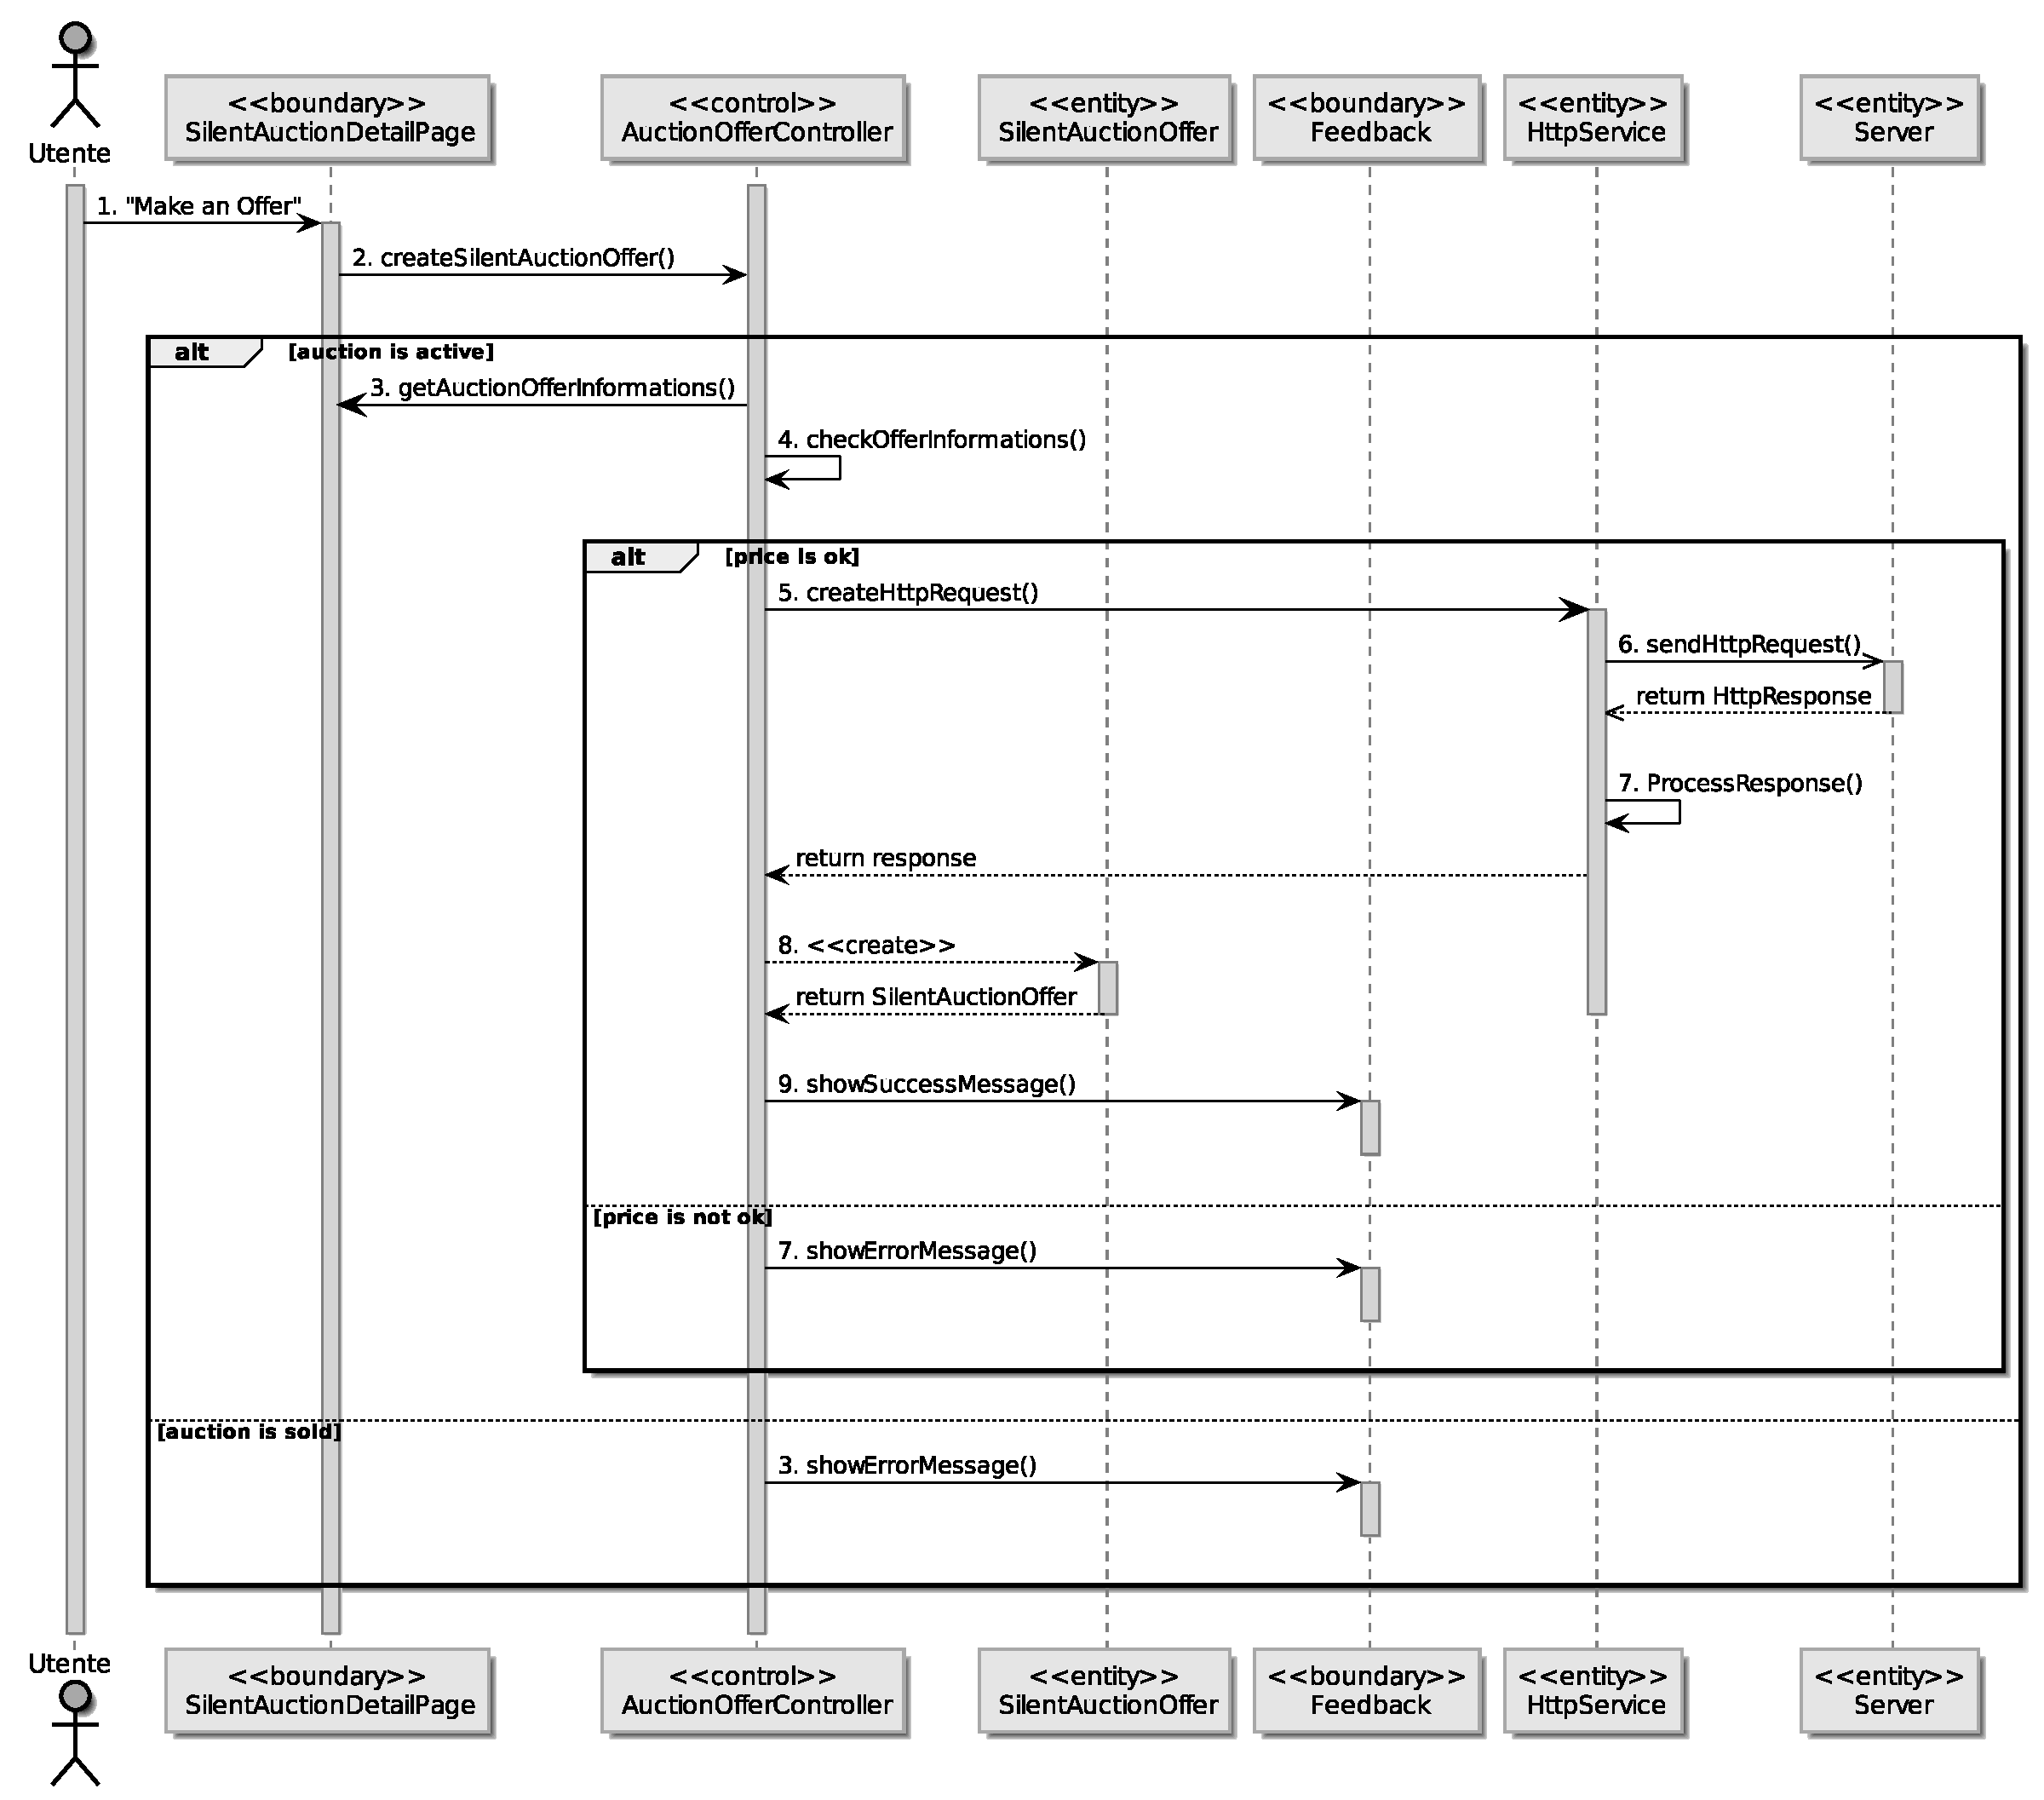
\includegraphics[width=\textwidth]{assets/sequence/piazzare_offerta_asta_silenziosa.eps}

\subsection{Caso d'uso: Aggiunta Link Social}
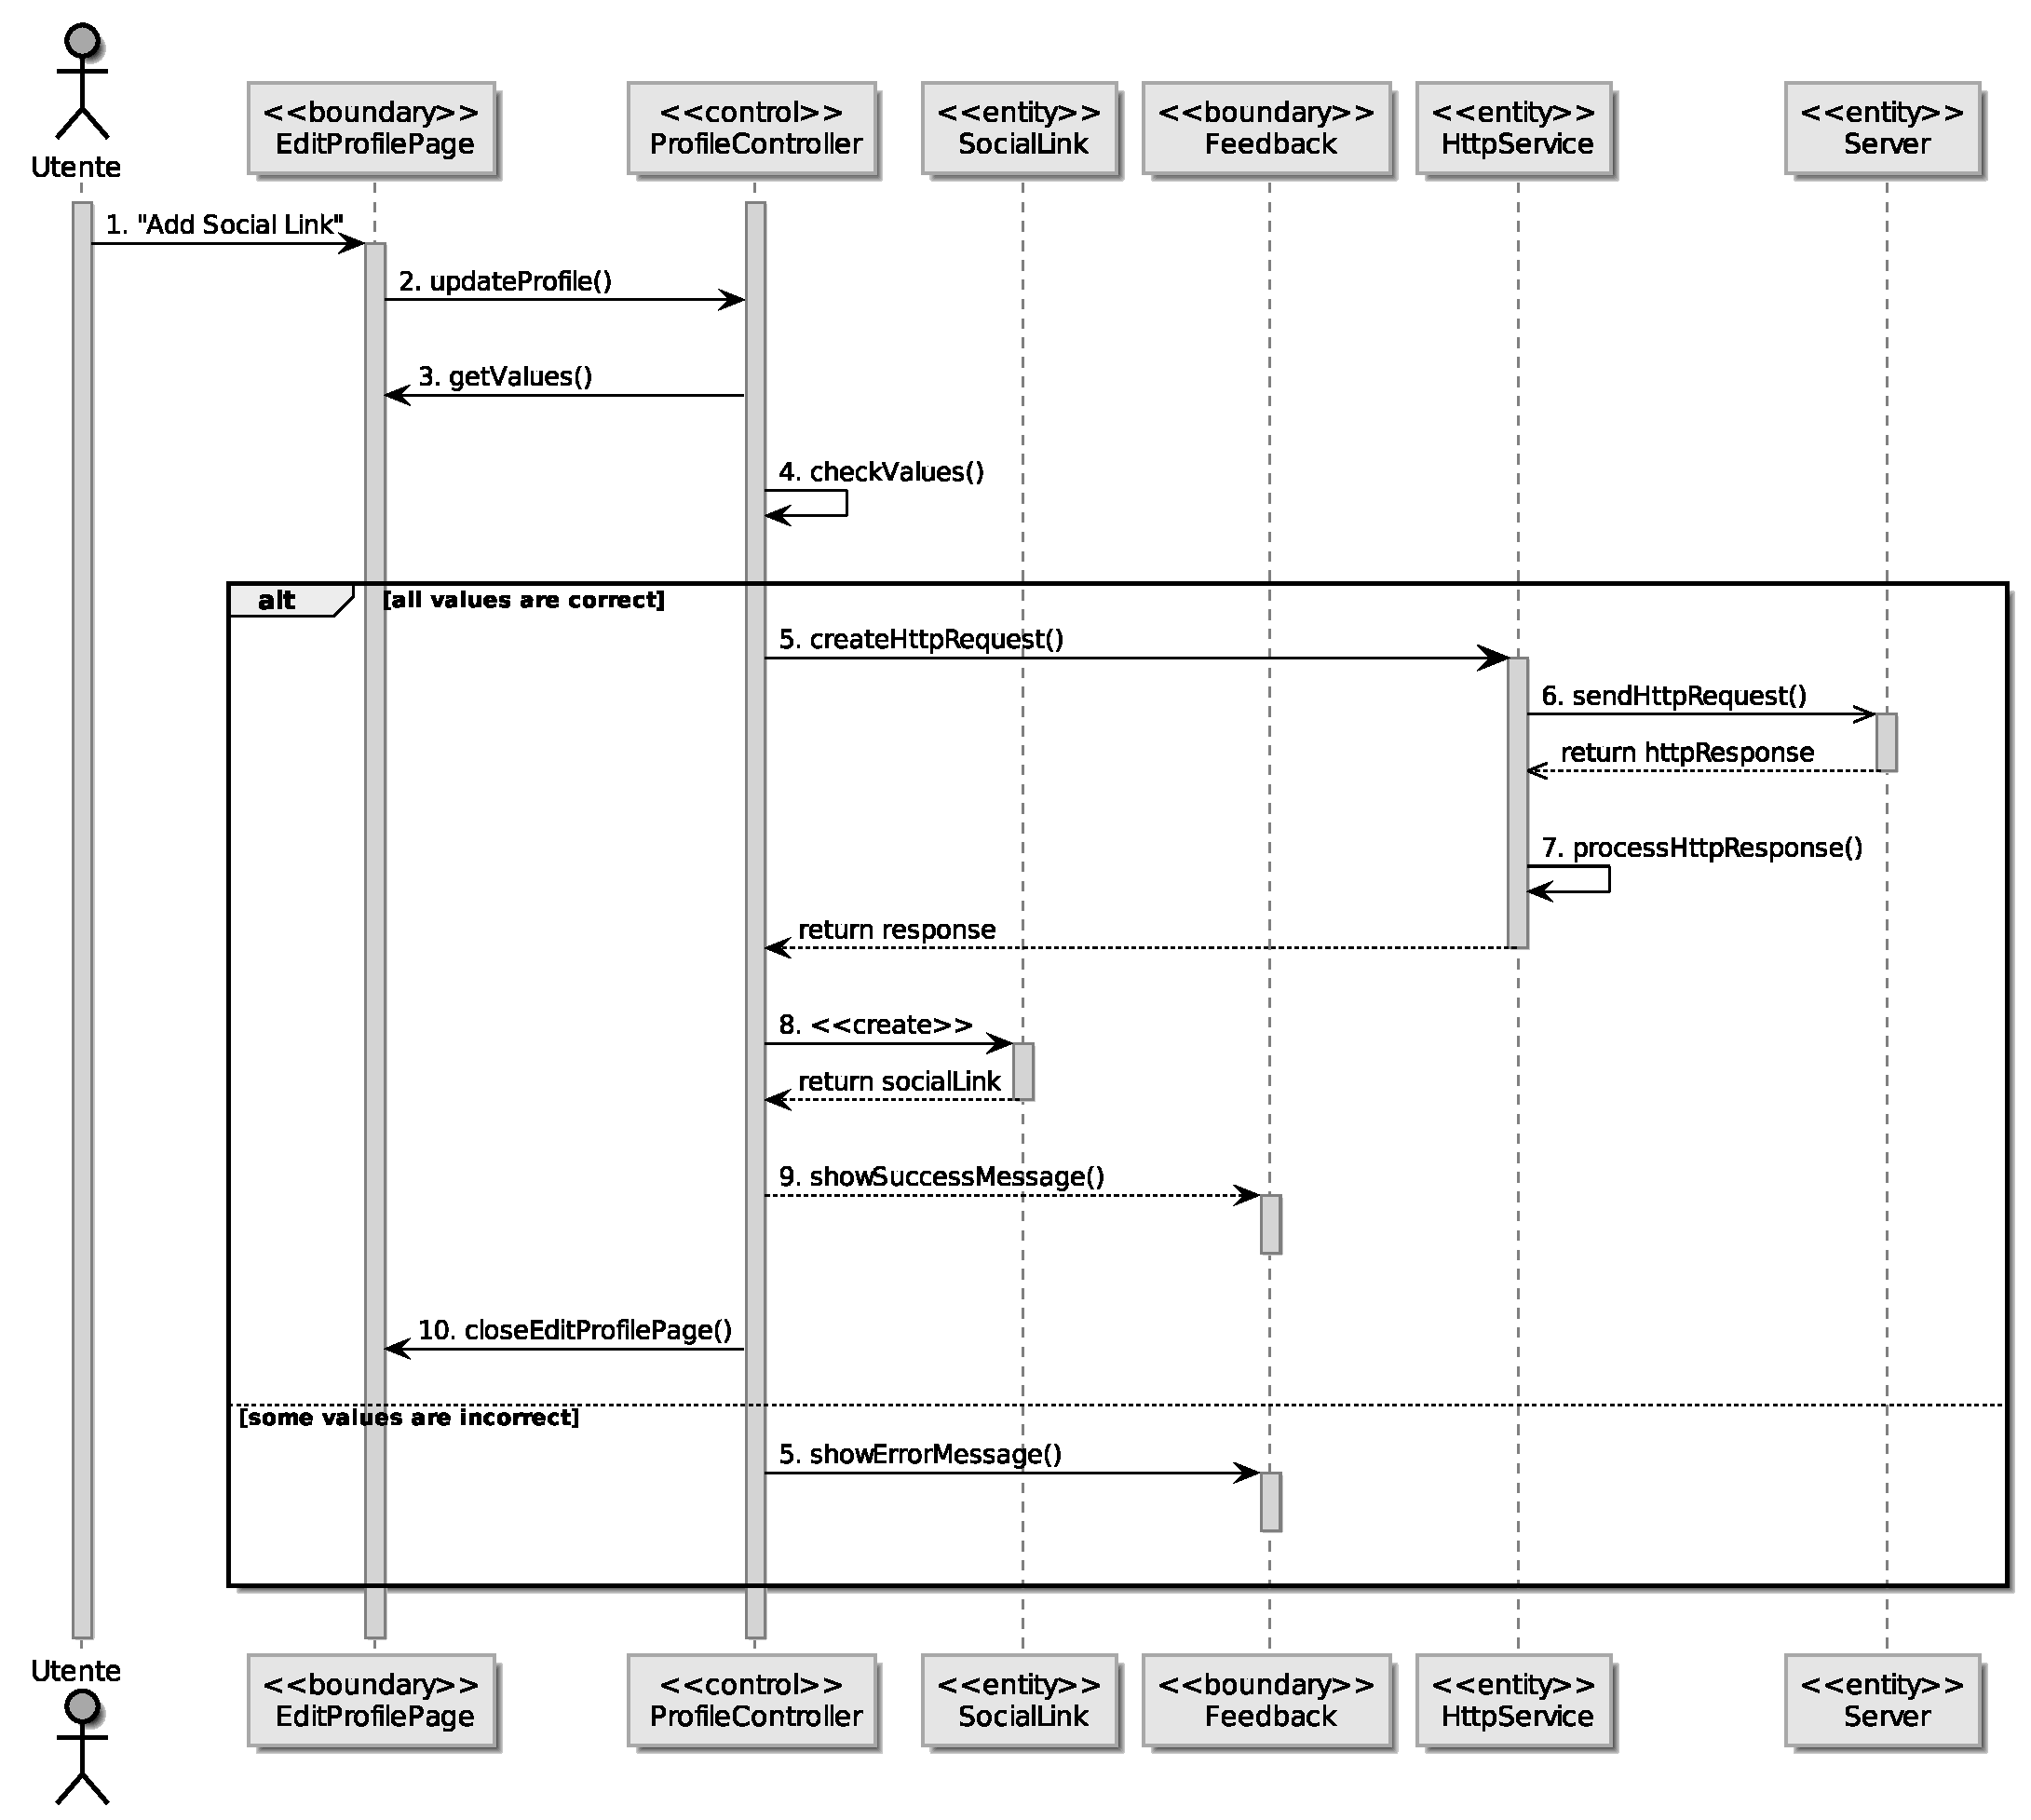
\includegraphics[width=\textwidth]{assets/sequence/aggiungere_link_social.eps}

\subsection{Caso d'uso: Storico Aste create}
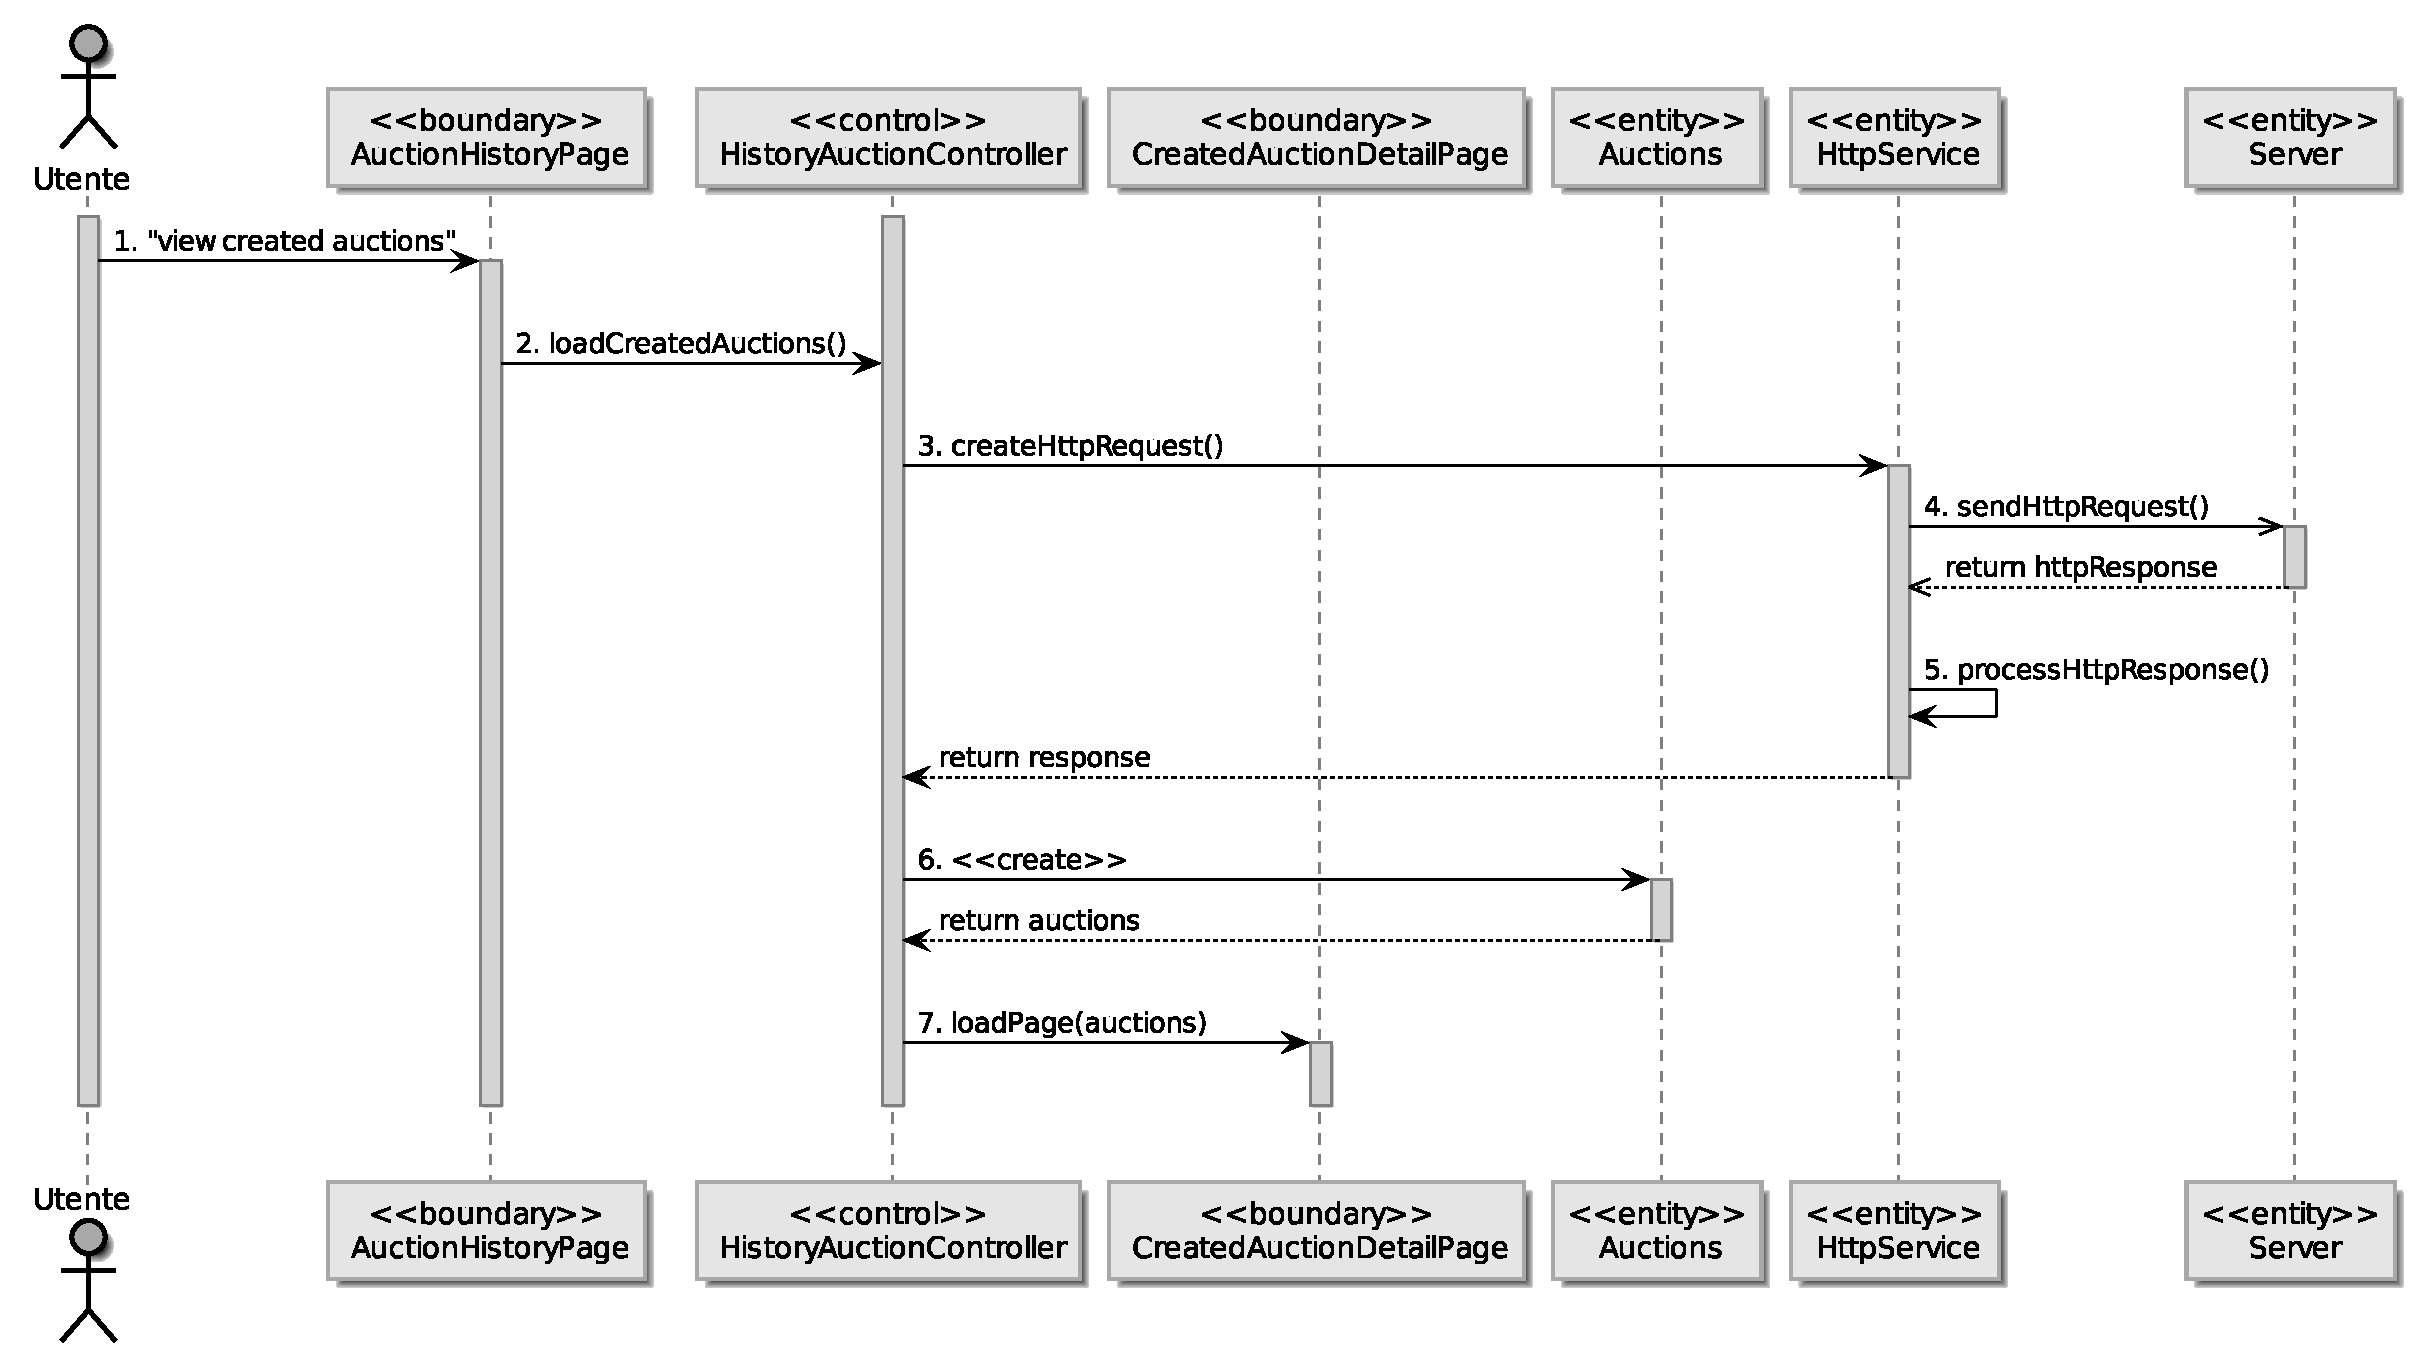
\includegraphics[width=\textwidth]{assets/sequence/visualizzazione_storico_aste_ancora_attive.eps}
